\documentclass{article}[10pt]
\usepackage[pdftex]{graphicx}
\usepackage{amsfonts}
\usepackage[italian]{babel}
\usepackage{graphicx}

%****************enlarge layout
\textheight     243.5mm
\topmargin      -20.0mm
\textwidth      480pt
\hoffset        -80pt
%*****************theorems and such
\newcounter{esnu}
\newenvironment{esercizio}{\medskip \noindent {\bf Esercizio\addtocounter{esnu}{1} \arabic{esnu}}}{}
\pagestyle{empty}
\newcommand{\liff}{\mathrel{\leftrightarrow}}   % Logical IFF Symbol
\newcommand{\metaiff}{\Longleftrightarrow}      %iff in metatheory

\begin{document}

%\begin{tabular}{llclcr}
% \hspace{-35pt} &{\bf COGNOME:} & \hspace{100pt}        &{\bf NOME:}    & \hspace{100pt}        &{\bf MATRICOLA:}%\hspace{35pt} \\
%\hline
%\end{tabular}
\begin{center} {\bf Esame di Programmazione II, 30 settembre 2015}\end{center}
%\`

Un sistema per visualizzare e modificare un orario \`e organizzato secondo lo schema
model/view/controller. Il modello contiene le informazioni sull'orario e pu\`o essere
legato a una o pi\`u view, che ne mostrano il contenuto:

{\scriptsize\begin{verbatim}
public interface Model {
  void linkToView(View view); // connette il modello a una view
  void set(int hours, int minutes, int seconds) throws IllegalArgumentException; // modifica ora, minuti e secondi
  int getHours();
  int getMinutes();
  int getSeconds();
}
\end{verbatim}}

\begin{esercizio}
\textbf{[4 punti]}
Si completi la seguente implementazione del modello, senza dimenticare di lanciare l'eccezione
se l'orario \`e illegale (le ore devono essere valori
da 0 a 23 inclusi; i minuti e secondi da 0 a 59 inclusi):

{\scriptsize\begin{verbatim}
public class Time implements Model {
  ...
  private final Set<View> views = new HashSet<>(); // tutte le view a cui e' connesso

  @Override
  public void set(int hours, int minutes, int seconds) throws IllegalArgumentException {
    ...
    for (View view: views)  // notifica tutte le view del nuovo orario
      view.onTimeChanged(hours, minutes, seconds);
  }
  ...
  @Override
  public void linkToView(View view) {
    views.add(view);
    view.onTimeChanged(hours, minutes, seconds);
  }
}
\end{verbatim}}
\end{esercizio}

\begin{esercizio}
\textbf{[4 punti]}
Una view visualizza l'orario ed \`e notificata di ogni suo cambiamento:

{\scriptsize\begin{verbatim}
public interface View {
  void onTimeChanged(int hours, int minutes, int seconds);
}
\end{verbatim}}

\noindent
Se ne realizzi l'implementazione \texttt{TextDateView} che, ad ogni cambiamento dell'orario,
stampa sul video un messaggio del tipo \texttt{15:05:09} oppure
\texttt{1:05:19}. Si osservi, in questi due esempi,
dove vanno messi gli \texttt{0} e dove invece non vanno messi e si scriva il codice
di conseguenza.
\end{esercizio}

\begin{esercizio}
\textbf{[5 punti]}
Un controllore riceve ordini di modifica dell'orario e li implementa sul modello:

{\scriptsize\begin{verbatim}
public interface Controller {
  void onIncreaseHours(); // e' stato richiesto l'incremento (circolare) dell'ora
  void onDecreaseHours(); // e' stato richiesto il decremento (circolare) dell'ora
  void onIncreaseMinutes(); // e' stato richiesto l'incremento (circolare) dei minuti
  void onDecreaseMinutes(); // e' stato richiesto il decremento (circolare) dei minuti
  void onIncreaseSeconds(); // e' stato richiesto l'incremento (circolare) dei secondi
  void onDecreaseSeconds(); // e' stato richiesto il decremento (circolare) dei secondi
  void onResetTime(); // e' stato richiesto di resettare l'orario al momento corrente
}
\end{verbatim}}

\noindent
Se ne completi l'implementazione seguente:

{\scriptsize\begin{verbatim}
public class ControllerImpl implements Controller {
  private final Model model; // dove effettuare le modifiche

  public ControllerImpl(Model model) {
    this.model = model;
    onResetTime(); // alla creazione del controller, il modello viene settato al tempo corrente
  }
  ...
  @Override
  public void onResetTime() {
    Calendar calendar = Calendar.getInstance();
    model.set(calendar.get(Calendar.HOUR_OF_DAY), calendar.get(Calendar.MINUTE), calendar.get(Calendar.SECOND));
  }
}
\end{verbatim}}
\end{esercizio}

\newpage
\begin{esercizio}\textbf{[9 punti]}
Una versione grafica della view pu\`o essere realizzata tramite la libreria Swing, includendo anche dei
bottoni per incrementare e decrementare le tre componenti dell'orario, come nel disegno seguente:

\begin{center}
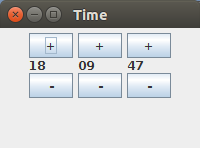
\includegraphics[width=5cm]{SwingDateView}
\end{center}

\noindent
Per esempio si pu\`o usare il seguente codice:

{\scriptsize\begin{verbatim}
public class SwingDateView extends JFrame implements View {
  private final JLabel hours = new JLabel(), minutes = new JLabel(), seconds = new JLabel();

  public SwingDateView(Controller controller) {
    super("Time"); setMinimumSize(new Dimension(200, 120));
    add(buildClockPanel(controller), BorderLayout.CENTER);  // aggiunge le componenti grafiche necessarie
    pack(); setVisible(true);
  }

  protected JPanel buildClockPanel(Controller controller) {
    JPanel clock = new JPanel();

    // crea la colonna delle ore
    JPanel hoursPanel = new JPanel();
    hoursPanel.setLayout(new BorderLayout());
    JButton increaseHours = new JButton("+");
    hoursPanel.add(increaseHours, BorderLayout.NORTH);
    hoursPanel.add(hours, BorderLayout.CENTER);
    JButton decreaseHours = new JButton("-");
    hoursPanel.add(decreaseHours, BorderLayout.SOUTH);
    clock.add(hoursPanel);
    ... codice simile per la colonna dei minuti e dei secondi: NON SCRIVETELO, TANTO E' IDENTICO

    // settaggio dei listeners di attivazione dei bottoni
    increaseHours.addActionListener(e -> controller.onIncreaseHours());
    decreaseHours.addActionListener(e -> controller.onDecreaseHours());
    increaseMinutes.addActionListener(e -> controller.onIncreaseMinutes());
    decreaseMinutes.addActionListener(e -> controller.onDecreaseMinutes());
    increaseSeconds.addActionListener(e -> controller.onIncreaseSeconds());
    decreaseSeconds.addActionListener(e -> controller.onDecreaseSeconds());

    return clock;
  }

  @Override
  public void onTimeChanged(int hours, int minutes, int seconds) {
    this.hours.setText(String.valueOf(hours));
    this.minutes.setText(String.format("%02d", minutes));
    this.seconds.setText(String.format("%02d", seconds));
  }
}
\end{verbatim}}

\noindent
Si scriva una estensione \texttt{Swing12DateView} di \texttt{SwingDateView}, che visualizza l'orario
nel formato a 12 ore inglese, in cui \emph{am} indica gli orari precedenti al mezzogiorno
e \emph{pm} indica gli orari dal mezzogiorno in poi.
Si ricordi che, in tale formato, il 12 sostituisce lo 0, per cui la mezzanotte \`e indicata
come 12am e il mezzogiorno come 12pm. L'estensione dovr\`a essere una componente grafica del tipo:

\begin{center}
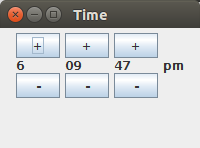
\includegraphics[width=5cm]{Swing12DateView}
\end{center}

\noindent
Ovviamente l'indicazione am/pm dovr\`a variare sulla base degli aggiornamenti di orario che
arrivano alla componente.
\end{esercizio}

\end{document}
